%!TEX root=/home/ska124/Dropbox/Thesis/thes-full.tex

%%%%%%%%%%%%%%%%%%%%%%%%%%%%%%%%%%%%%%%%%%%%%%%%%
%
%     Chapter 6
%
%%%%%%%%%%%%%%%%%%%%%%%%%%%%%%%%%%%%%%%%%%%%%%%%

\chapter{Detour: Europarl}
\label{chap:europarl}

\section{What is Europarl?}
Europarl refers to the parallel corpora generated by translating the proceedings of European parliament into several languages. Version 7 of Europarl now has 20 languages, from French to Estonian and Finnish. Release of the Europarl corpus led to a surge in research into more and more data-driven methods to enable Statistical Machine Translation. The results were easily reproducible and the data is very clean and sentence-aligned. 

Moreover, Europarl is multi-parallel. What does multi-parallel imply? Consider english as the common target language. A multi-parallel corpora between 20 European languages and English comprises sentences in 20 european languages which translate to the same english sentence. 

\begin{figure}
	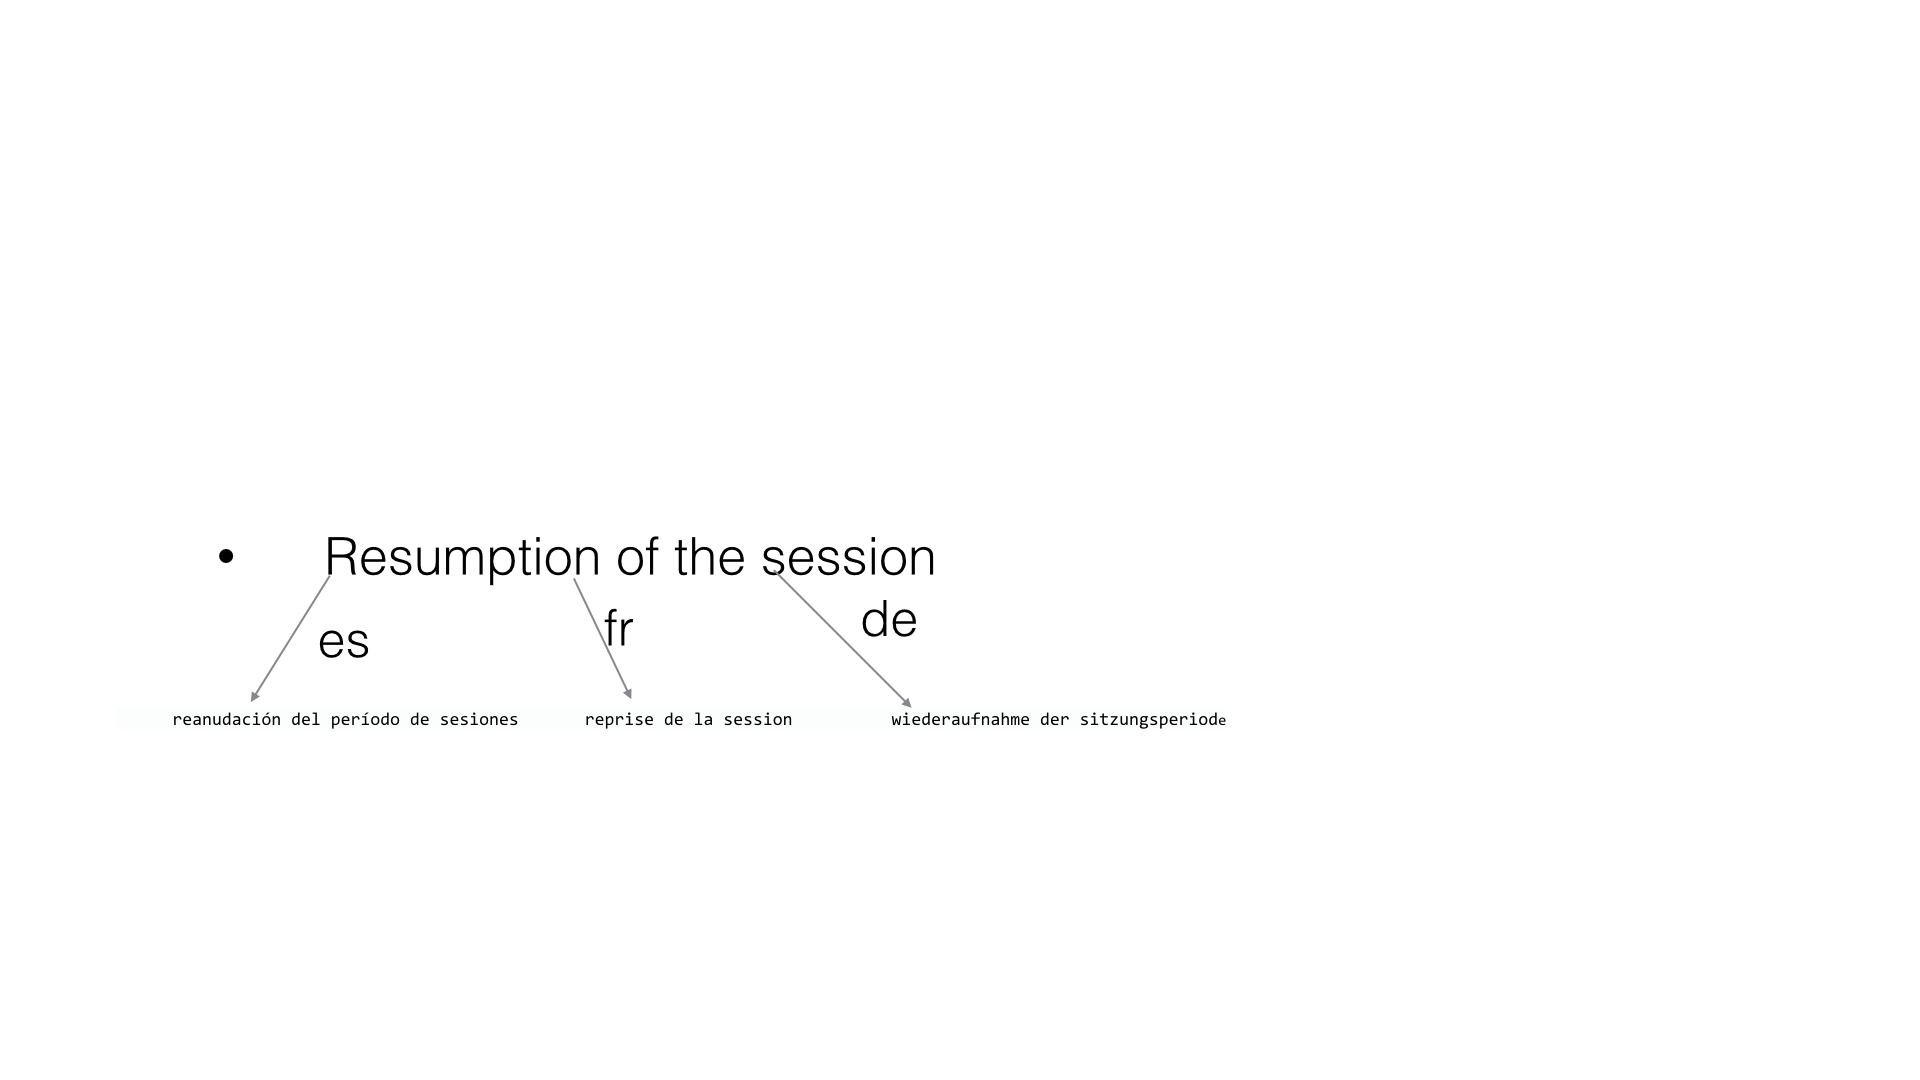
\includegraphics[scale=0.4]{files/Figures/eparl_multiparallel.jpg}
	\caption{Spanish = es, French = fr, German = de}
	\label{fig:eparl_multi}
\end{figure}


\section{Triangulation for Europarl languages}



\section{How best to simulate low-resource?}

~\cite{Cohn:07} simulated ``low-resource'' settings by using the top 10K sentences for the source pivot, pivot target and source target systems.  

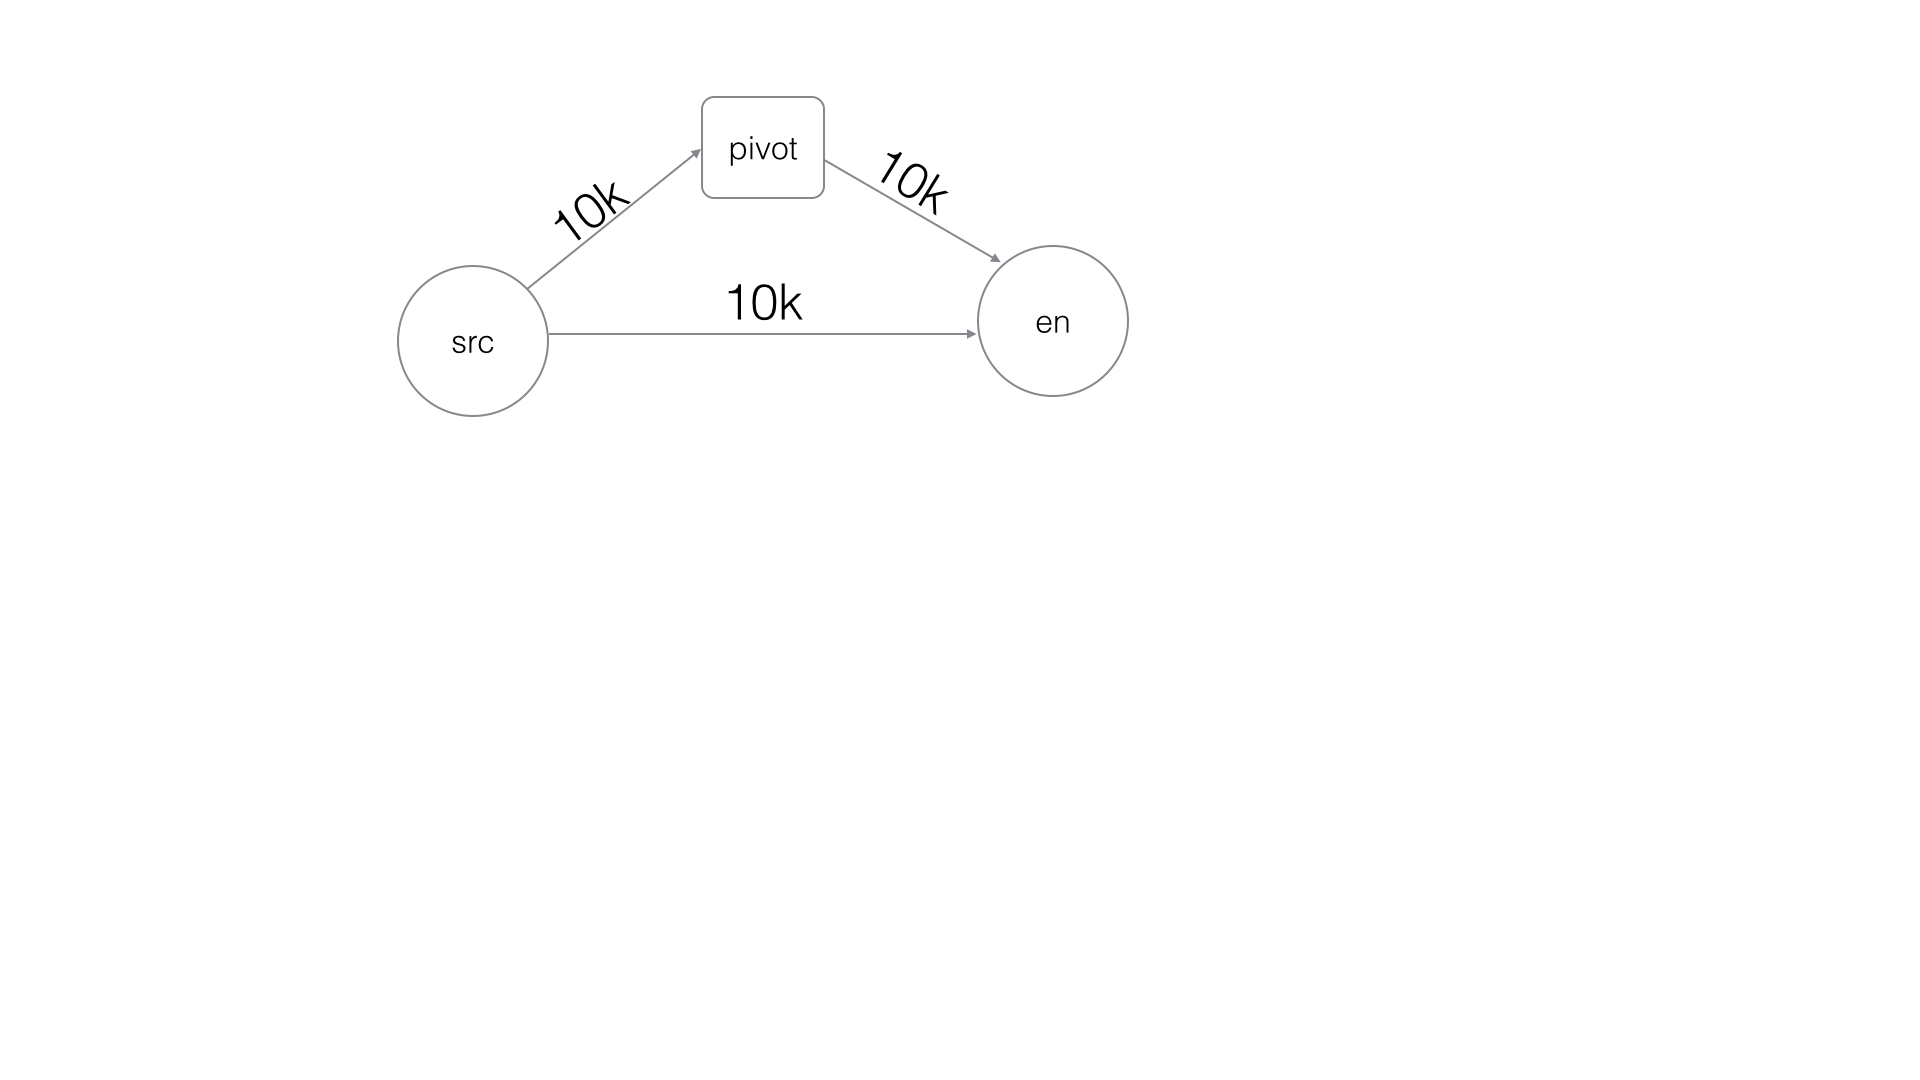
\includegraphics[scale=0.2]{files/Figures/Cohn.jpg} \\
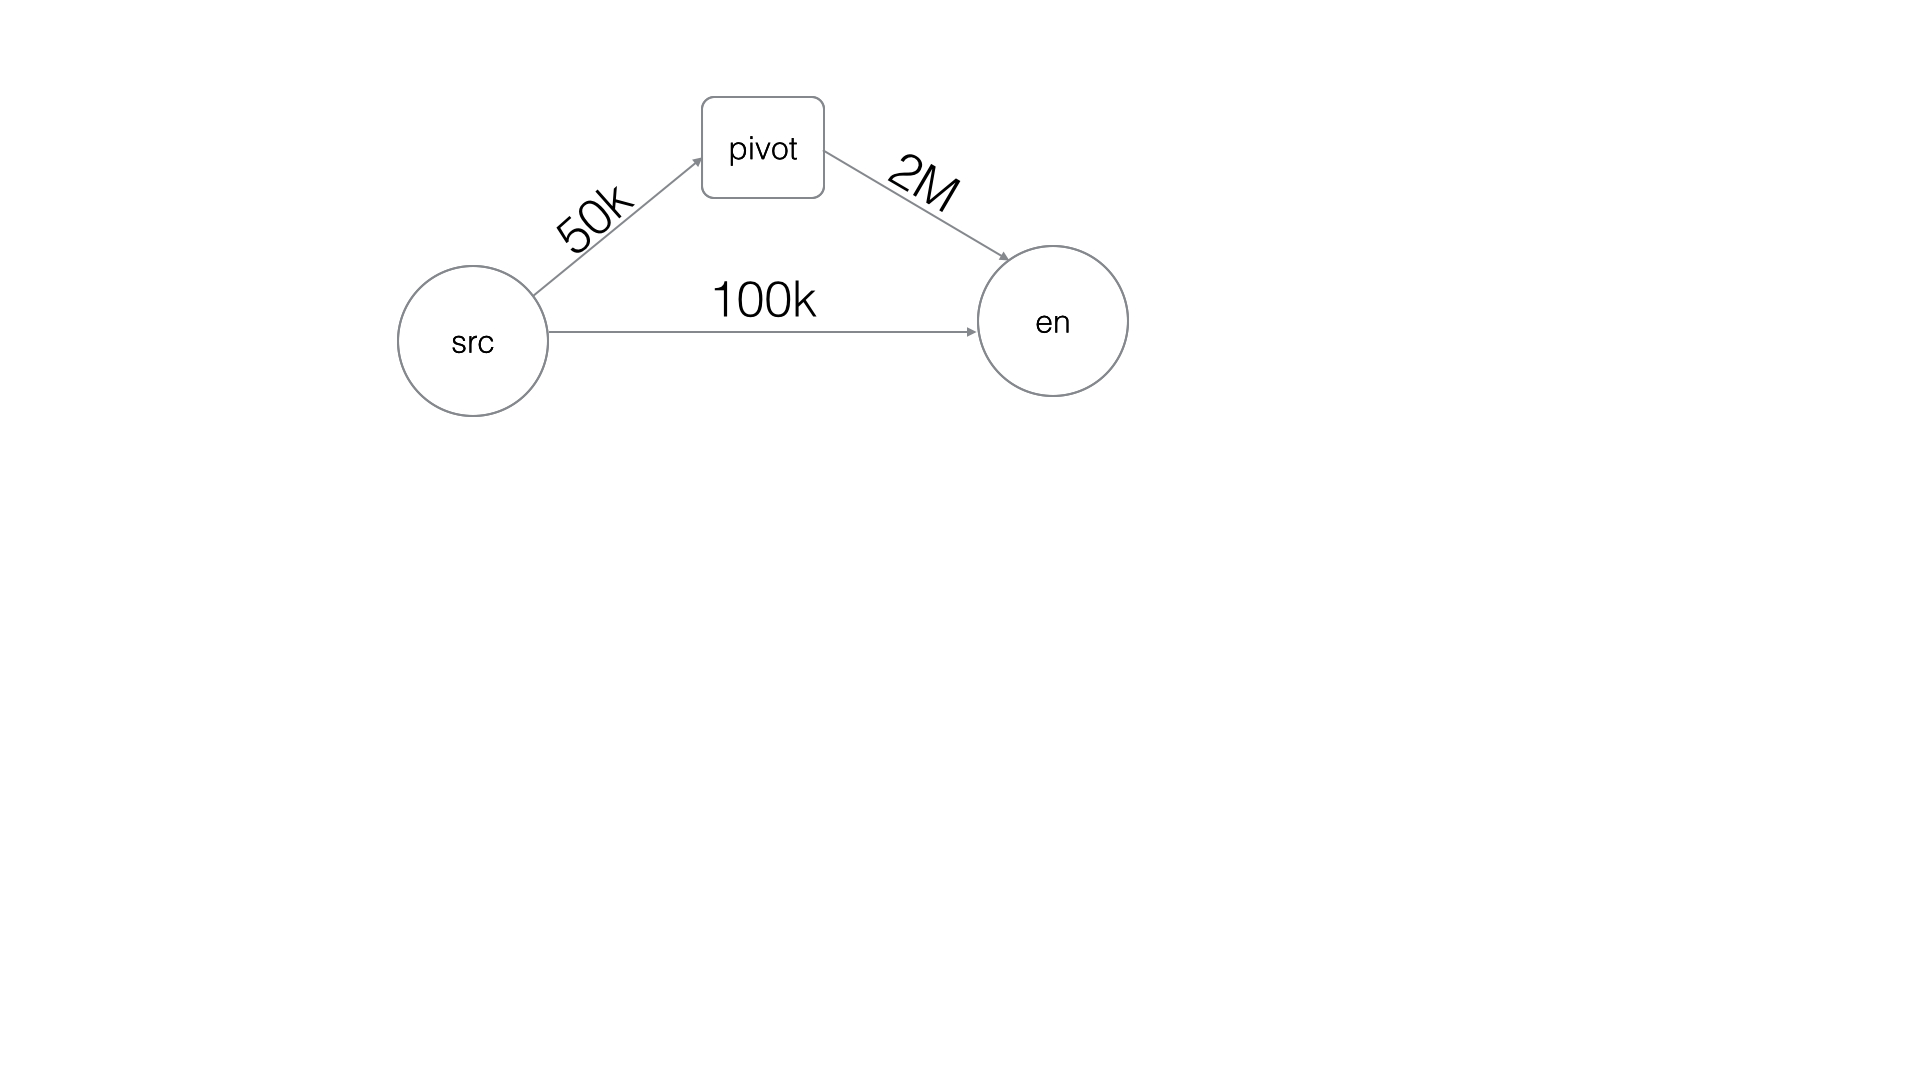
\includegraphics[scale=0.2]{files/Figures/Our.jpg} \\

\section{Experiments}
\begin{tabular}{lr}

\toprule
System & BLEU \\
\toprule
es-en & 23.32 \\
fr-en & 19.53 \\
de-en & 15.60 \\
\bottomrule
\centering
\small
\label{table:eparl100}
\end{tabular} \\
\begin{tabular}{lrrrrrr}
\toprule

src-tgt & pivot & top20 & top40 & top60 & top80 & top100 \\
\toprule

de-en & fr & 13.32 & 13.33 & 13.35 & 13.42 & 13.03 \\
de-en & es & 13.37 & 13.17 & 13.49 & 13.34 & 13.36 \\
fr-en & de & 16.21 & 15.82 & 15.89 & 16.08 & - \\
fr-en & es & 17.77 & 18.15 & 17.99 & 18.01 & 18.27 \\
es-en & fr & 21.35 & 21.18 & 20.83 & 21.01 & 21.45\\
es-en & de & 18.36 & 19.19 & 19.35 & 19.23 & 18.97 \\
\bottomrule
\centering 
\small
\label{table:eparltopn}
\end{tabular}
 \\

\section{Remarks}









